\documentclass[journal,12pt,twocolumn]{IEEEtran}

\usepackage{setspace}
\usepackage{gensymb}
\singlespacing
\usepackage[cmex10]{amsmath}

\usepackage{amsthm}

\usepackage{mathrsfs}
\usepackage{txfonts}
\usepackage{stfloats}
\usepackage{bm}
\usepackage{cite}
\usepackage{cases}
\usepackage{subfig}

\usepackage{longtable}
\usepackage{multirow}

\usepackage{enumitem}
\usepackage{mathtools}
\usepackage{steinmetz}
\usepackage{tikz}
\usepackage{circuitikz}
\usepackage{verbatim}
\usepackage{tfrupee}
\usepackage[breaklinks=true]{hyperref}
\usepackage{graphicx}
\usepackage{tkz-euclide}

\usetikzlibrary{calc,math}
\usepackage{listings}
    \usepackage{color}                                            %%
    \usepackage{array}                                            %%
    \usepackage{longtable}                                        %%
    \usepackage{calc}                                             %%
    \usepackage{multirow}                                         %%
    \usepackage{hhline}                                           %%
    \usepackage{ifthen}                                           %%
    \usepackage{lscape}     
\usepackage{multicol}
\usepackage{chngcntr}

\DeclareMathOperator*{\Res}{Res}

\renewcommand\thesection{\arabic{section}}
\renewcommand\thesubsection{\thesection.\arabic{subsection}}
\renewcommand\thesubsubsection{\thesubsection.\arabic{subsubsection}}

\renewcommand\thesectiondis{\arabic{section}}
\renewcommand\thesubsectiondis{\thesectiondis.\arabic{subsection}}
\renewcommand\thesubsubsectiondis{\thesubsectiondis.\arabic{subsubsection}}


\hyphenation{op-tical net-works semi-conduc-tor}
\def\inputGnumericTable{}                                 %%

\lstset{
%language=C,
frame=single, 
breaklines=true,
columns=fullflexible
}
\begin{document}


\newtheorem{theorem}{Theorem}[section]
\newtheorem{problem}{Problem}
\newtheorem{proposition}{Proposition}[section]
\newtheorem{lemma}{Lemma}[section]
\newtheorem{corollary}[theorem]{Corollary}
\newtheorem{example}{Example}[section]
\newtheorem{definition}[problem]{Definition}

\newcommand{\BEQA}{\begin{eqnarray}}
\newcommand{\EEQA}{\end{eqnarray}}
\newcommand{\define}{\stackrel{\triangle}{=}}
\bibliographystyle{IEEEtran}
\raggedbottom
\setlength{\parindent}{0pt}
\providecommand{\mbf}{\mathbf}
\providecommand{\pr}[1]{\ensuremath{\Pr\left(#1\right)}}
\providecommand{\qfunc}[1]{\ensuremath{Q\left(#1\right)}}
\providecommand{\sbrak}[1]{\ensuremath{{}\left[#1\right]}}
\providecommand{\lsbrak}[1]{\ensuremath{{}\left[#1\right.}}
\providecommand{\rsbrak}[1]{\ensuremath{{}\left.#1\right]}}
\providecommand{\brak}[1]{\ensuremath{\left(#1\right)}}
\providecommand{\lbrak}[1]{\ensuremath{\left(#1\right.}}
\providecommand{\rbrak}[1]{\ensuremath{\left.#1\right)}}
\providecommand{\cbrak}[1]{\ensuremath{\left\{#1\right\}}}
\providecommand{\lcbrak}[1]{\ensuremath{\left\{#1\right.}}
\providecommand{\rcbrak}[1]{\ensuremath{\left.#1\right\}}}
\theoremstyle{remark}
\newtheorem{rem}{Remark}
\newcommand{\sgn}{\mathop{\mathrm{sgn}}}
\providecommand{\abs}[1]{\left\vert#1\right\vert}
\providecommand{\res}[1]{\Res\displaylimits_{#1}} 
\providecommand{\norm}[1]{\left\lVert#1\right\rVert}
%\providecommand{\norm}[1]{\lVert#1\rVert}
\providecommand{\mtx}[1]{\mathbf{#1}}
\providecommand{\mean}[1]{E\left[ #1 \right]}
\providecommand{\fourier}{\overset{\mathcal{F}}{ \rightleftharpoons}}
%\providecommand{\hilbert}{\overset{\mathcal{H}}{ \rightleftharpoons}}
\providecommand{\system}{\overset{\mathcal{H}}{ \longleftrightarrow}}
	%\newcommand{\solution}[2]{\textbf{Solution:}{#1}}
\newcommand{\solution}{\noindent \textbf{Solution: }}
\newcommand{\cosec}{\,\text{cosec}\,}
\providecommand{\dec}[2]{\ensuremath{\overset{#1}{\underset{#2}{\gtrless}}}}
\newcommand{\myvec}[1]{\ensuremath{\begin{pmatrix}#1\end{pmatrix}}}
\newcommand{\mydet}[1]{\ensuremath{\begin{vmatrix}#1\end{vmatrix}}}
\numberwithin{equation}{subsection}
\makeatletter
\@addtoreset{figure}{problem}
\makeatother
\let\StandardTheFigure\thefigure
\let\vec\mathbf
\renewcommand{\thefigure}{\theproblem}
\def\putbox#1#2#3{\makebox[0in][l]{\makebox[#1][l]{}\raisebox{\baselineskip}[0in][0in]{\raisebox{#2}[0in][0in]{#3}}}}
     \def\rightbox#1{\makebox[0in][r]{#1}}
     \def\centbox#1{\makebox[0in]{#1}}
     \def\topbox#1{\raisebox{-\baselineskip}[0in][0in]{#1}}
     \def\midbox#1{\raisebox{-0.5\baselineskip}[0in][0in]{#1}}
\vspace{3cm}
\title{C $\&$ DS Assignment}
\author{ADYASA MOHANTY - EE18BTECH11048}
\maketitle
\newpage
\bigskip
\renewcommand{\thefigure}{\theenumi}
\renewcommand{\thetable}{\theenumi}
Download codes from 
\begin{lstlisting}
https://github.com/adyasa611/EE4013/tree/main/Assignment-1/codes
\end{lstlisting}
%
and latex-tikz codes from 
%
\begin{lstlisting}
https://github.com/adyasa611/EE4013/tree/main/Assignment-1/figures
\end{lstlisting}
\section{\textbf{Solving a circuit problem using Graph Theory}}
 

\begin{figure}[h!]
    \centering
    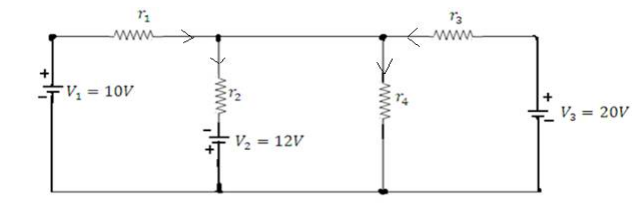
\includegraphics[width=9cm]{img_1.png}
    \caption{Question}
    \label{fig:Question}
\end{figure}
$r_1=2 \ohm, r_2=5 \ohm, r_3=1 \ohm,r_4=10 \ohm$

\section{\textbf{Theory}}


\subsection{Fundamental Tie Set Matrix (Fundamental Loop Matrix)}

\begin{enumerate}
\item We define the edges of the graph and remove all the elements like voltage source, resistor, capacitor from the circuit and the corresponding graph is formed.

\item The graph has loops, we define and number the edges and the non overlapping loops and give a direction for current flow in each loop.

\item We then form a matrix with n (number of edges) rows and m (number of loops) columns.
\item We check if an edge is a part of the loop or not, if it is not then we assign 0 in the respective cell.
\item If edge is part of the loop, we check the direction of loop and current flow. If they coincide we assign the value 1 in the cell, else -1.
\item This is the Fundamental Tie Set Matrix, denoted by B.
\end{enumerate}

\subsection{KVL $\&$ KCL}

\begin{enumerate}
\item KVL states that for a closed loop series path the algebraic sum of all the voltages around any closed loop in a circuit is equal to zero.
\item In the matrix form it can be represented as $B$ $V_b$=$0$ where $V_b$ vector represents the total voltage drop in each branch of the circuit(edge).
\item $V_b = V_s + Z_bI_b$ where $V_s, Z_b, I_b $ are matrices and vectors
\item $V_s$= Voltage Source, $I_b$= Current in that branch, $Z_b$= Impedance of that branch.
\item $B(V_s + Z_bI_b) = 0$
\item $B(Z_bI_b) = -BV_s$
\item From KCL we know that $I_b=B^TI_L$ where $B^T$ is the transpose of B and $I_L$ is the current in each loop.
\item So, $BZ_bB^TI_L = -BV_s$
\end{enumerate}


\section{\textbf{Solution for given Circuit}}

\begin{enumerate}
\item The graph for the given circuit can be represented as:

\begin{figure}[h!]
    \centering
    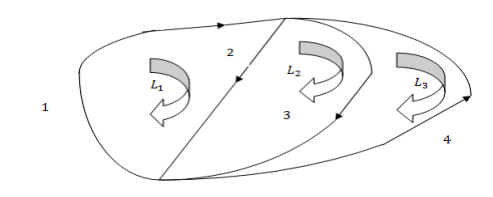
\includegraphics[width=9cm]{img_2.png}
    \caption{Loops and Current Flow}
    \label{Loops and Current Flow}
\end{figure}

\item We have to define the parameters
\[ B=
      \begin{bmatrix}
        1 & 1 & 0 & 0\\
        0 & -1 & 1 & 0\\
        0 & 0 & -1 & -1 \\
        \end{bmatrix}

\[ Z_b =
\begin{bmatrix}
        2 & 0 & 0 & 0\\
        0 & 5 & 0 & 0\\
        0 & 0 & 1 & 0 \\
        0 & 0 & 0 & 10\\
        \end{bmatrix}

\[ V_s =
\begin{bmatrix}
    10\\
    12\\
    0 \\
    20\\
    \end{bmatrix}\quad

\[I_L =
\begin{bmatrix}
    $I_1$\\
    $I_2$\\
    $I_3$\\
    \end{bmatrix}

\item We put these parameters in the equation : $BZ_bB^TI_L = -BV_s$



\item We can solve this using pen and paper or using a basic code.

Python code to solve the above equation.
\begin{lstlisting}
codes/Circuit.py
\end{lstlisting}
\item The current values are
$I_L =$
\begin{bmatrix}
    $-3.72A$\\
    $-0.8A$\\
    $1.74A$\\
    \end{bmatrix}
\item The negative sign indicates that our assumption of current flow direction was wrong.
\end{enumerate}
\end{document}